%% This is an example first chapter.  You should put chapter/appendix that you
%% write into a separate file, and add a line \include{yourfilename} to
%% main.tex, where `yourfilename.tex' is the name of the chapter/appendix file.
%% You can process specific files by typing their names in at the 
%% \files=
%% prompt when you run the file main.tex through LaTeX.
\chapter{Experiments}\label{chap:exp}

\section{Evaluation criteria} \label{sec:evacri}
\subsection{Object detection metrics}
Average Precision is a standard and popular metric in measuring the performance of the object detection and segmentation algorithms. The Precision (Prcn) and Recall (Rcll) are defined as follow:
\begin{equation}
	Prcn = \frac{TP}{TP+FP}
\end{equation}
\begin{equation}
	Rcll = \frac{TP}{TP+FN}
\end{equation}
where, TP, FP, and FN are number of True Positive, False Positive, and False Negative, respectively. A predicted bounding box is considered a TP if its intersection over union (IoU), or Jaccard Index, with a ground truth box is larger than 0.5. Equation \ref{eq:IoU} shows how the IoU between a predicted box P and a ground truth box G is calculated.
\begin{equation}
	\label{eq:IoU}
	IoU(P,G) = \frac{|P\cap G|}{| P \cup G |}
\end{equation}
F1 score is a metric that combines recall and precision into a single score by calculating the harmonic mean of precision and recall:
\begin{equation}
	F1 = \frac{2TP}{2TP+FP+FN}
\end{equation}
Latest research papers tend to give results in the COCO dataset format. In COCO mAP, a 101-point interpolated AP definition is used in the calculation. For COCO, AP is the average over multiple IoU. AP@[. 5: .95] corresponds to the average AP for IoU from 0.5 to 0.95 with a step size of 0.05. The following are some other metrics collected for the COCO dataset:
\subsection{Object tracking metrics}
Performance is measured according to the framework presented in MOT16 \cite{DBLP:journals/corr/MilanL0RS16} and in the same manner as performance is measure in the MOTChallange. The authors of \cite{DBLP:journals/corr/MilanL0RS16} provide publicly available code for evaluation, this code is used to calculate the different performance metrics. MOT16 was chosen since it is a compilation of other many metrics developed in an attempt to standardize evaluation of multiple object tracking. MOT16 contains a wide array of metrics for evaluation of multiple object tracking, some which are quite similar to each other. Hence, metrics that were considered to similar to other have not been included in this thesis.
\begin{itemize}
	\item Identification Recall (IDR) and Identification Precision (IDP): IDR and IDP are similar to the metrics Recall and Precision for object detection. The metrics will however differ since objects are considered tracked only if they can be assigned an identity, which will not be the case for all detected objects. Another difference is that inconsistencies in identity assignments will lower the IDTP score. For each ground truth identity, the predicted identity most similar to it is found. Any other identity assigned to the ground truth identity is then considered a mismatch (IDFP) and will be counted as a false positive instead of a true positive.
	\begin{equation}
		IDR = \frac{IDTP}{IDTP+IDFP}
	\end{equation}
	\begin{equation}
		IDP = \frac{IDTP}{IDTP+IDFN}
	\end{equation}
where, IDTP is the sum of TP in detection and the number of correctly labeled objects in the tracking; IDFP/IDFN is the sum of FP/FN in detection and the number of correctly predicted objects for positive class in detection but incorrectly labeled in tracking.
	\item IDF1-score(IDF1): Similar to F1 score for object detection, IDF1 combines both IDR and IDP into a single score to facilitate comparisons of different trackers. The higher IDF1 is, the better tracker is.
	\begin{equation}
		IDF1 = \frac{2IDTP}{2IDTP+IDFP+IDFN}
	\end{equation}
	\item Mostly Tracked (MT): The number of ground truth identities that are tracked for 80\% or more of their existence.
	\item Partly Tracked (PT): The number of ground truth identities that are tracked between 20\% and 80\% of their existence.
	\item Mostly Lost (ML): The number of ground truth identities that are tracked for less than 20\% of their existence.
	\item Identity Switches (IDs): The number of identity switches. An identity switch is counted every time an already tracked ground truth identity is assigned a new tracking identity.
	\item Track Fragmentations (FM): The number of track fragmentations. A track fragmentation is counted every time a tracked ground truth identity is lost and then found again in a later frame.
	\item Multiple Object Tracking Accuracy (MOTA): MOTA combines false negatives, false positives and identity switches into a single score in order to express overall performance with a single value. This is the most important metric for object tracking evaluation and it is defined as:
	\begin{equation}
		MOTA = 1 - \frac{\sum _t (IDFN_t+IDFP_t+IDS_t)}{\sum _t GT_t}
	\end{equation}
where, t is the index of frame, GT is the number of objserved objects in the real-world. It is worth to note that MOTA would be a negative value if there are many errors in the tracking process and the number of these errors is larger than that of observed objects.
	\item Multiple Object Tracking Precision(MOTP): MOTP measures how well correctly predicted bounding boxes TP fit their respective ground truth boxes GT. This is done by calculating the average overlap between true positives and their corresponding ground truth object.
	\begin{equation}
		MOTP = \frac{\sum _t d_{t,i}}{\sum _t c_t}
	\end{equation}
where, \(c_t\) denotes the number of matches found in the frame t and \(d_{t,i}\) is the sum of distances between all true positive and their corresponding ground truth i. This metric indicate the ability of the tracking in estimating precise object positions.
\end{itemize}
\section{Experimental results}
The following sub-sections will present result for different object detection and tracking algorithms tested in this thesis. All experiments are conducted on 32 videos of Micand32 datasets. The average inference speed is measured on a Workstation supermicro with Intel® Xeon®, CPU E5-2620 v2@2.1GHz, 6 cores, 12 threads, RAM 12GB, GPU GTX 1080.
\subsection{Egocentric hand detection and segmentation result}\label{subsec:det_res}
This subsection presents results for the different object detection algorithms consider in this thesis. The algorithms to be evaluated are: Yolov3\_spp, Yolov4x, FasterRCNN\_R\_50\_FPN\_3x, MaskRCNN\_R\_50\_FPN\_3x. Detection evaluation is show in Table \ref{tab:detres_ap}, Table \ref{tab:detres_ar} and Table \ref{tab:detres_sp}.
\begin{table}[]
	\centering
	\label{tab:detres_ap}
	\begin{tabular}{|l|l|l|l|l|l|l|}
		\hline
		Algorithm                  & AP            & AP50          & AP75          & \(AP^{small}\) & \(AP^{medium}\)      & \(AP^{large}\)       \\ \hline
		Yolov3\_spp                & 89.2          & 92.4          & 92.1          & 1.1     & 66.4          & 54.1          \\ \hline
		Yolov4x                    & 93.1          & 95.6          & 94.6          & 3.2     & 72.5          & 42.9          \\ \hline
		FasterRCNN & \textbf{96.2} & 97.9          & \textbf{97.9} & 0.9     & \textbf{75.8} & 6.3           \\ \hline
		MaskRCNN  & 92.1          & \textbf{98.9} & 97.9          & 0.0     & 32.4          & \textbf{92.2} \\ \hline
	\end{tabular}
	\caption{Object detection and segmentation Average Precision following the COCO standard.}
\end{table}
\begin{table}[]
	\centering
	\resizebox{\textwidth}{!}{%
		\begin{tabular}{|l|l|l|l|l|l|l|}
			\hline
			Algorithm                  & \(AR^{max=1}\)      & \(AR^{max}=10\)      & \(AR^{max}=100\)     & \(AR^{small}\) & \(AR^{medium}\)      & \(AR^{large}\)       \\ \hline
			Yolov3\_spp                & 6.5          & 53.6          & 76.4          & 3.2     & 32.5          & 75.9          \\ \hline
			Yolov4x                    & 8.7          & 65.8          & 89.7          & 7.1     & 40.1          & 82.7          \\ \hline
			FasterRCNN\_R\_50\_FPN\_3x & \textbf{9.6} & 76.8          & \textbf{97.6} & 10.0    & \textbf{77.8} & \textbf{97.6} \\ \hline
			MaskRCNN\_R\_50\_FPN\_3x   & 9.2          & \textbf{73.9} & 94.6          & 0.0     & 50.8          & 94.7          \\ \hline
		\end{tabular}%
	}
	\caption{Object detection and segmentation Average Recall following the COCO standard.}
	\label{tab:detres_ar}
\end{table}
\begin{table}[hbt!]
	\centering
	\resizebox{\textwidth}{!}{%
		\begin{tabular}{|l|l|l|l|l|l|}
			\hline
			\multirow{2}{*}{Algorithm} & \multicolumn{2}{l|}{Average time}         & \multirow{2}{*}{Speed (Hz)} & \multicolumn{2}{l|}{Memory requirement (MB)} \\ \cline{2-3} \cline{5-6} 
			& Training (hour) & Inference (millisecond) &                             & RAM                   & GPU                  \\ \hline
			Yolov3\_spp                & \textbf{36}     & 45                      & 22                          & \textbf{1989}         & 2260                 \\ \hline
			Yolov4x                    & 40              & \textbf{38}             & \textbf{25}                 & 2152                  & \textbf{2076}        \\ \hline
			FasterRCNN\_R\_50\_FPN\_3x & 46              & 84                      & 12                          & 2351                  & 3297                 \\ \hline
			MaskRCNN\_R\_50\_FPN\_3x   & 50              & \textbf{215}            & \textbf{5}                  & \textbf{2461}         & \textbf{3674}        \\ \hline
		\end{tabular}%
	}
	\caption{Object detection and segmentation average training and inference time, speed and machine requirements.}
	\label{tab:detres_sp}
\end{table}
\subsection{Egocentric hand tracking result}
Tracking results for SORT and DeepSORT with different object detection strategy are presented in this section. As described in section 3.4, the tests are performed in a tracking by detection system where tracking and detection algorithms are completely separated. Therefore, different results for combinations of tracking and detection algorithms are reported. Further, ground-truth detections are also test with SORT and DeepSORT, this is done so as to give an insight how much of the error is due to the object detection algorithm and how much of it is due to the tracking algorithm. Tracking performance with ground-truth detections should only have errors introduced by the tracking algorithms and can thereby give an upper limit for how much better the tracking by detection system can become by changing object detection algorithm. Thus, this frameworks consists of 6 detction and segmentation algorithms, they are: Yolov3\_SPP, Yolov4x, Faster\_RCNN\_R\_50\_FPN\_3x, Mask\_RCNN\_R50\_FPN\_3x, Mask\_RCNN\_R50\_FPN\_3x with region based and detection ground-truth. Their combination with 2 tracking algorithms, SORT and DeepSORT, we obtain a total of 12 options for the pipeline. However, the combination of MaskRCNN with region based and SORT scheme is identical to the combination of Mask and SORT scheme because in theory, the SORT algorithm does not use visual information fields. To conclude, we have 11 approaches conventionally defined as in the Table \ref{tab:notation} for brief presentation.
\begin{table}[]
	\centering
	\label{tab:notation}
	\begin{tabular}{|l|l|l|l|}
		\hline
		No & Detector              & Tracker                                        & Notation \\ \hline
		1  & Yolov3                & \multirow{5}{*}{SORT}                          & Y3S      \\ \cline{1-2} \cline{4-4} 
		2  & Yolov4                &                                                & Y4S      \\ \cline{1-2} \cline{4-4} 
		3  & FasterRCNN            &                                                & FS       \\ \cline{1-2} \cline{4-4} 
		4  & MaskRCNN              &                                                & MS       \\ \cline{1-2} \cline{4-4} 
		5  & Groundtruth           &                                                & GS       \\ \hline
		6  & Yolov3                & \multicolumn{1}{c|}{\multirow{6}{*}{DeepSORT}} & Y3DS     \\ \cline{1-2} \cline{4-4} 
		7  & Yolov4                & \multicolumn{1}{c|}{}                          & Y4DS     \\ \cline{1-2} \cline{4-4} 
		8  & FasterRCNN            & \multicolumn{1}{c|}{}                          & FS       \\ \cline{1-2} \cline{4-4} 
		9  & MaskRCNN              & \multicolumn{1}{c|}{}                          & MS       \\ \cline{1-2} \cline{4-4} 
		10 & MaskRCNN+Region based & \multicolumn{1}{c|}{}                          & RDS      \\ \cline{1-2} \cline{4-4} 
		11 & Groundtruth           & \multicolumn{1}{c|}{}                          & GDS      \\ \hline
	\end{tabular}
	\caption{Notation of the 11 approaches mentioned and used in the experiments.}
	\vspace{-0.7cm}
\end{table}
\\In this thesis, I conduct the experiments to evaluate the performance of these approaches on the custom dataset Micand32 which contains 2 sub-datasets: Micand32S and Micand32E. The properties of this dataset is reported in chapter \ref{chap:method}, sub-section \ref{subsec:micand32}.
\subsubsection{Short-term tracking on a standard dataset: Micand32S}
The Mican32S sub-datasets contains 26 sequences containing in total 3162 frames as per the MOT16 Challenge rules and recommendations, each containing from 100 to 300 images. These recordings are chosen so every video has an excursion span of precisely one patient’s activity, for instance opening the cap of the water bottle, getting the circle, playing with ball, turning left of right, etc. Simultaneously, every video generally contains just 1 or 2 active hands. This sub-dataset can be characterized into short-term tracking datasets. The desire set for the framework proposed in this theory is to recognize, segment, and track this entire fundamental excursion of the hand. Since the quantity of recordings is up to 26 recordings, in this part I will list the overall evaluation for each approach on the whole 26 recordings, which is a weighted average of the quantity of frames per video. Besides, I likewise measure a case of 26 recordings running on 1 approach to see the impact of the sort of activity on the presentation of the framework. Note that the hand in the 26 recordings is utilized to train the deep appearance descriptor for DeepSORT as referenced in chapter \ref{chap:framework}, sub-section \ref{subsec:train_deep}. Table \ref{tab:short_overall} reports short-term tracking overall result on Micand32S following the MOT16 evaluation protocol.
% Please add the following required packages to your document preamble:
% \usepackage{graphicx}
% Please add the following required packages to your document preamble:
% \usepackage{graphicx}
% Please add the following required packages to your document preamble:
% \usepackage{graphicx}
% Please add the following required packages to your document preamble:
% \usepackage{graphicx}
\begin{table}[]
	\centering
	\resizebox{\textwidth}{!}{%
		\begin{tabular}{|l|l|l|l|l|l|l|l|l|l|l|l|l|l|l|l|}
			\hline
			Method & \begin{tabular}[c]{@{}l@{}}IDF1\\ (\%)$\uparrow$­\end{tabular} & 
			\begin{tabular}[c]{@{}l@{}}IDP\\ (\%)$\uparrow$­\end{tabular} & 
			\begin{tabular}[c]{@{}l@{}}IDR\\ (\%)$\uparrow$­\end{tabular} & 
			\begin{tabular}[c]{@{}l@{}}Rcll\\$\uparrow$    ­\end{tabular} & 
			\begin{tabular}[c]{@{}l@{}}Prcn\\$\uparrow$    ­\end{tabular} & 
			\begin{tabular}[c]{@{}l@{}}GT\\$\uparrow$      ­\end{tabular} & 
			\begin{tabular}[c]{@{}l@{}}MT\\$\uparrow$      ­\end{tabular} & 
			\begin{tabular}[c]{@{}l@{}}PT\\$\uparrow$      ­\end{tabular} &
			\begin{tabular}[c]{@{}l@{}}ML\\$\downarrow$     \end{tabular} &
			\begin{tabular}[c]{@{}l@{}}FP\\$\downarrow$     \end{tabular} &        
			\begin{tabular}[c]{@{}l@{}}FN\\$\downarrow$     \end{tabular} &         
			\begin{tabular}[c]{@{}l@{}}IDs\\$\downarrow$     \end{tabular} &        
			\begin{tabular}[c]{@{}l@{}}FM\\$\downarrow$     \end{tabular} &         
			\begin{tabular}[c]{@{}l@{}}\textbf{MOTA}\\ (\%)$\uparrow$­\end{tabular} &
			\begin{tabular}[c]{@{}l@{}}MOTP\\ $\downarrow$­\end{tabular}            \\ \hline
			Y3S    & 97.0                                                 & 99.6                                                & 94.6                                                & 94.8                                                   & 99.8                                                   & 35                                                   & 33          & \textbf{1}                                           & 1          & 6          & 207        & 1          & 1          & 94.6                                                 & 0.087          \\ \hline
			Y4S    & 98.6                                                 & 99.4                                                & 97.7                                                & 97.8                                                   & 99.4                                                   & 35                                                   & \textbf{34} & \textbf{1}                                           & \textbf{0} & 23         & 89         & \textbf{0} & 5          & 97.2                                                 & 0.108          \\ \hline
			FS     & 97.1                                                 & 99.7                                                & 94.6                                                & 94.8                                                   & 99.9                                                   & 35                                                   & 33          & \textbf{1}                                           & 1          & 4          & 206        & 1          & 1          & 94.7                                                 & 0.087          \\ \hline
			MS     & 98.8                                                 & 99.7                                                & 98.0                                                & 98.2                                                   & 99.9                                                   & 35                                                   & 34          & \textbf{1}                                           & \textbf{0} & 3          & 73         & 1          & 1          & 98.1                                                 & 0.072          \\ \hline
			GS     & \textbf{99.9}                                        & 99.9                                                & \textbf{99.9}                                       & \textbf{99.9}                                          & \textbf{100.0}                                         & 35                                                   & \textbf{34} & \textbf{1}                                           & \textbf{0} & 1          & 4          & \textbf{0} & \textbf{0} & \textbf{99.9}                                        & 0.089          \\ \hline
			Y3DS   & 97.1                                                 & 99.6                                                & 94.7                                                & 94.9                                                   & 99.8                                                   & 35                                                   & 33          & \textbf{1}                                           & 1          & 7          & 203        & 1          & 2          & 94.7                                                 & 0.088          \\ \hline
			Y4DS   & 98.8                                                 & 99.6                                                & 97.9                                                & 98.1                                                   & 99.8                                                   & 35                                                   & \textbf{34} & \textbf{1}                                           & \textbf{0} & 7          & 74         & 1          & 2          & 97.9                                                 & 0.106          \\ \hline
			FDS    & 98.2                                                 & 99.9                                                & 96.5                                                & 96.5                                                   & \textbf{100.0}                                         & 35                                                   & 33          & \textbf{1}                                           & 1          & 1          & 140        & \textbf{0} & \textbf{0} & 96.5                                                 & 0.077          \\ \hline
			MDS    & 98.2                                                 & 99.9                                                & 96.5                                                & 96.5                                                   & \textbf{100.0}                                         & 35                                                   & 33          & \textbf{1}                                           & 1          & 1          & 140        & \textbf{0} & \textbf{0} & 96.5                                                 & 0.076          \\ \hline
			RDS    & 99.3                                                 & 99.3                                                & 99.3                                                & 99.3                                                   & 99.4                                                   & 35                                                   & \textbf{34} & \textbf{1}                                           & \textbf{0} & 25         & 27         & \textbf{0} & 6          & 98.7                                                 & 0.089          \\ \hline
			GDS    & \textbf{99.9}                                        & \textbf{100}                                        & 99.8                                                & 99.8                                                   & \textbf{100.0}                                         & 35                                                   & \textbf{34} & \textbf{1}                                           & \textbf{0} & \textbf{0} & \textbf{0} & \textbf{0} & 1          & 99.8                                                 & \textbf{0.062} \\ \hline
		\end{tabular}%
	}
	\caption{Short-term tracking \textbf{overall} result on Micand32S following the MOT16 evaluation protocol.}
	\label{tab:short_overall}
\end{table}
The GDS presents an alomost perfect performance on Micand32S, detailed metrics of this method is revealed in Figure \ref{fig:GDS_short}. Of all ground-truth-free approaches, the Y4DS approach reaches a remarkable result shown in Figure \ref{fig:y4ds_short}.
\subsubsection{Long-term tracking on a realistic dataset: Micand32E}
In this part, I wil validate the effectiveness of the 11 approaches on the Micand32E dataset. As referenced in chapter \ref{chap:method}, sub-section \ref{subsec:micand32}, the Micand32E contains 6 sequences, the sequence length of each is in range of 1000 frames and 2000 frames, and total the volume of this sub-dataset is 7857 frames. Also, this sub-dataset fully contains 4 types of patient’s action: (5) practice with ball, (6) practice with water bottles, (7) practice with wooden blocks, (8) practice with cylinders. This sub-dataset is very releastic, interesting and quite challenging because it is specifically selected with careful observations  by developers in the NAFOSTED’s project who are experienced in computer vision problems.
Table \ref{tab:long_overall} presents the overall tracking results inferenced on Micand32E of the 11 approaches.
% Please add the following required packages to your document preamble:
% \usepackage{graphicx}
% Please add the following required packages to your document preamble:
% \usepackage{graphicx}
\begin{table}[]
	\centering
	\resizebox{\textwidth}{!}{%
		\begin{tabular}{|l|l|l|l|l|l|l|l|l|l|l|l|l|l|l|l|}
			\hline
			Method & \begin{tabular}[c]{@{}l@{}}IDF1\\ (\%)$\uparrow$­\end{tabular} & 
			\begin{tabular}[c]{@{}l@{}}IDP\\ (\%)$\uparrow$­\end{tabular} & 
			\begin{tabular}[c]{@{}l@{}}IDR\\ (\%)$\uparrow$­\end{tabular} & 
			\begin{tabular}[c]{@{}l@{}}Rcll\\$\uparrow$    ­\end{tabular} & 
			\begin{tabular}[c]{@{}l@{}}Prcn\\$\uparrow$    ­\end{tabular} & 
			\begin{tabular}[c]{@{}l@{}}GT\\$\uparrow$      ­\end{tabular} & 
			\begin{tabular}[c]{@{}l@{}}MT\\$\uparrow$      ­\end{tabular} & 
			\begin{tabular}[c]{@{}l@{}}PT\\$\uparrow$      ­\end{tabular} &
			\begin{tabular}[c]{@{}l@{}}ML\\$\downarrow$     \end{tabular} &
			\begin{tabular}[c]{@{}l@{}}FP\\$\downarrow$     \end{tabular} &        
			\begin{tabular}[c]{@{}l@{}}FN\\$\downarrow$     \end{tabular} &         
			\begin{tabular}[c]{@{}l@{}}IDs\\$\downarrow$     \end{tabular} &        
			\begin{tabular}[c]{@{}l@{}}FM\\$\downarrow$     \end{tabular} &         
			\begin{tabular}[c]{@{}l@{}}\textbf{MOTA}\\ (\%)$\uparrow$­\end{tabular} &
			\begin{tabular}[c]{@{}l@{}}MOTP\\ $\downarrow$­\end{tabular}            \\ \hline 
			Y3S    & 51.4          & 59.4          & 45.2          & 75.3                                                   & 99.4                                                   & 24   & 7                                                    & 8                                                    & 9                                                    & 68                                                   & 3630                                                 & 123                                                   & 174                                                  & 74.1          & 0.133          \\ \hline
			Y4S    & 56.7          & 60.7          & 53.0          & 86.4                                                   & 99.4                                                   & 24   & 9                                                    & \textbf{11}                                          & 4                                                    & 81                                                   & 1996                                                 & 134                                                   & 159                                                  & 85.0          & 0.127          \\ \hline
			FS     & 74.5          & 73.9          & 74.8          & 97.9                                                   & 97.1                                                   & 24   & 17                                                   & 7                                                    & \textbf{0}                                           & 426                                                  & 306                                                  & 115                                                   & 91                                                   & 94.2          & 0.082          \\ \hline
			MS     & 74.5          & 73.9          & 74.8          & 97.9                                                   & 97.2                                                   & 24   & 17                                                   & 7                                                    & \textbf{0}                                           & 420                                                  & 304                                                  & 114                                                   & 90                                                   & 94.3          & 0.082          \\ \hline
			GS     & 89.1          & 89.3          & 88.7          & 98.5                                                   & 99.6                                                   & 24   & 21                                                   & 3                                                    & \textbf{0}                                           & 62                                                   & 220                                                  & 91                                                    & 50                                                   & 97.5          & 0.059          \\ \hline
			Y3DS   & 58.7          & 66.0          & 52.6          & 78.4                                                   & 98.7                                                   & 24   & 9                                                    & 7                                                    & 8                                                    & 149                                                  & 3176                                                 & 123                                                   & 202                                                  & 76.6          & 0.151          \\ \hline
			Y4DS   & 65.0          & 68.1          & 61.9          & 89.3                                                   & 98.5                                                   & 24   & 11                                                   & 9                                                    & 4                                                    & 194                                                  & 1581                                                 & 122                                                   & 192                                                  & 87.1          & 0.142          \\ \hline
			FDS    & 79.4          & 79.0          & 79.5          & 98.1                                                   & 97.8                                                   & 24   & 17                                                   & 7                                                    & \textbf{0}                                           & 320                                                  & 282                                                  & 117                                                   & 75                                                   & 95.1          & 0.060          \\ \hline
			MDS    & 83.5          & 83.5          & 83.3          & 98.1                                                   & 98.7                                                   & 24   & 18                                                   & 5                                                    & 1                                                    & 184                                                  & 275                                                  & 95                                                    & 61                                                   & 96.2          & 0.054          \\ \hline
			RDS    & \textbf{89.6} & \textbf{89.5} & \textbf{89.5} & 98.2                                                   & 98.6                                                   & 24   & 16                                                   & 8                                                    & \textbf{0}                                           & 212                                                  & 258                                                  & 79                                                    & 74                                                   & 96.3          & 0.072          \\ \hline
			GDS    & 88.5          & 88.5          & 88.1          & \textbf{99.1}                                          & \textbf{99.9}                                          & 24   & \textbf{23}                                          & 1                                                    & \textbf{0}                                           & \textbf{12}                                          & \textbf{135}                                         & 82                                                    & \textbf{43}                                          & \textbf{98.4} & \textbf{0.052} \\ \hline
		\end{tabular}%
	}
	\caption{Long-term tracking \textbf{overrall} results on Micand32E following the MOT16 protocol.}
	\label{tab:long_overall}
\end{table}
To analyze the complexity and the difficulty of the four types of action, I analyzed the results of the tracking algorithm that achives highest MOTA, the GDS, across these four action types. This result is shown in the Table \ref{tab:long_gds}.
% Please add the following required packages to your document preamble:
% \usepackage{graphicx}
\begin{table}[]
	\centering
	\resizebox{\textwidth}{!}{%
		\begin{tabular}{|l|l|l|l|l|l|l|l|l|l|l|l|l|l|l|l|}
			\hline
			Method & \begin{tabular}[c]{@{}l@{}}IDF1\\ (\%)$\uparrow$­\end{tabular} & 
			\begin{tabular}[c]{@{}l@{}}IDP\\ (\%)$\uparrow$­\end{tabular} & 
			\begin{tabular}[c]{@{}l@{}}IDR\\ (\%)$\uparrow$­\end{tabular} & 
			\begin{tabular}[c]{@{}l@{}}Rcll\\$\uparrow$    ­\end{tabular} & 
			\begin{tabular}[c]{@{}l@{}}Prcn\\$\uparrow$    ­\end{tabular} & 
			\begin{tabular}[c]{@{}l@{}}GT\\$\uparrow$      ­\end{tabular} & 
			\begin{tabular}[c]{@{}l@{}}MT\\$\uparrow$      ­\end{tabular} & 
			\begin{tabular}[c]{@{}l@{}}PT\\$\uparrow$      ­\end{tabular} &
			\begin{tabular}[c]{@{}l@{}}ML\\$\downarrow$     \end{tabular} &
			\begin{tabular}[c]{@{}l@{}}FP\\$\downarrow$     \end{tabular} &        
			\begin{tabular}[c]{@{}l@{}}FN\\$\downarrow$     \end{tabular} &         
			\begin{tabular}[c]{@{}l@{}}IDs\\$\downarrow$     \end{tabular} &        
			\begin{tabular}[c]{@{}l@{}}FM\\$\downarrow$     \end{tabular} &         
			\begin{tabular}[c]{@{}l@{}}\textbf{MOTA}\\ (\%)$\uparrow$­\end{tabular} &
			\begin{tabular}[c]{@{}l@{}}MOTP\\ $\downarrow$­\end{tabular}            \\ \hline 
			GH010354\_5\_17718\_19366 & 64.1          & 64.8          & 63.5          & 97.7                                                   & 99.6                                                   & 3          & 3                                                    & 0                                                    & \textbf{0}                                           & 7          & 41         & 5                                                     & 7                                                    & 97.0          & 0.096          \\ \hline
			GH010373\_5\_1284\_2724   & 89.1          & 89.1          & 88.7          & 98.8                                                   & 99.9                                                   & \textbf{6} & \textbf{6}                                           & 0                                                    & \textbf{0}                                           & 4          & 40         & 19                                                    & 14                                                   & 98.1          & 0.051          \\ \hline
			GH010358\_6\_10208\_11900 & 81.4          & 81.3          & 81.1          & 99.3                                                   & \textbf{100.0}                                         & 4          & 4                                                    & 0                                                    & \textbf{0}                                           & \textbf{0} & 24         & 8                                                     & 13                                                   & 99.0          & \textbf{0.038} \\ \hline
			GH010373\_6\_3150\_4744   & \textbf{99.7} & \textbf{99.8} & \textbf{99.5} & \textbf{99.8}                                          & \textbf{100.0}                                         & 4          & 4                                                    & 0                                                    & \textbf{0}                                           & \textbf{0} & 8          & \textbf{1}                                            & 1                                                    & \textbf{99.7} & 0.048          \\ \hline
			GH010358\_7\_2490\_3390   & 97.6          & 97.4          & 97.2          & 99.0                                                   & 99.9                                                   & 4          & 3                                                    & \textbf{1}                                           & \textbf{0}                                           & 1          & 19         & 9                                                     & 8                                                    & 98.5          & 0.050          \\ \hline
			GH010358\_8\_8000\_8547   & 97.2          & 97.3          & 97.0          & 99.7                                                   & \textbf{100.0}                                         & 3          & 3                                                    & 0                                                    & \textbf{0}                                           & \textbf{0} & \textbf{3} & 40                                                    & \textbf{0}                                           & 96.1          & 0.048          \\ \hline
			Overall                   & 88.5          & 88.5          & 88.1          & 99.1                                                   & 99.9                                                   & 24         & 23                                                   & 1                                                    & 0                                                    & 12         & 135        & 82                                                    & 43                                                   & 98.4          & 0.052          \\ \hline
		\end{tabular}%
	}
	\caption{GDS \textbf{detail} results on Micand32E.}
	\label{tab:long_gds}
\end{table}
Especially, the approach proposed by the author of this thesis performs an impressive result as in the Table \ref{tab:long_rds}.
\begin{table}[]
	\centering
	\resizebox{\textwidth}{!}{%
		\begin{tabular}{|l|l|l|l|l|l|l|l|l|l|l|l|l|l|l|l|}
			\hline
			Method & \begin{tabular}[c]{@{}l@{}}IDF1\\ (\%)$\uparrow$­\end{tabular} & 
			\begin{tabular}[c]{@{}l@{}}IDP\\ (\%)$\uparrow$­\end{tabular} & 
			\begin{tabular}[c]{@{}l@{}}IDR\\ (\%)$\uparrow$­\end{tabular} & 
			\begin{tabular}[c]{@{}l@{}}Rcll\\$\uparrow$    ­\end{tabular} & 
			\begin{tabular}[c]{@{}l@{}}Prcn\\$\uparrow$    ­\end{tabular} & 
			\begin{tabular}[c]{@{}l@{}}GT\\$\uparrow$      ­\end{tabular} & 
			\begin{tabular}[c]{@{}l@{}}MT\\$\uparrow$      ­\end{tabular} & 
			\begin{tabular}[c]{@{}l@{}}PT\\$\uparrow$      ­\end{tabular} &
			\begin{tabular}[c]{@{}l@{}}ML\\$\downarrow$     \end{tabular} &
			\begin{tabular}[c]{@{}l@{}}FP\\$\downarrow$     \end{tabular} &        
			\begin{tabular}[c]{@{}l@{}}FN\\$\downarrow$     \end{tabular} &         
			\begin{tabular}[c]{@{}l@{}}IDs\\$\downarrow$     \end{tabular} &        
			\begin{tabular}[c]{@{}l@{}}FM\\$\downarrow$     \end{tabular} &         
			\begin{tabular}[c]{@{}l@{}}\textbf{MOTA}\\ (\%)$\uparrow$­\end{tabular} &
			\begin{tabular}[c]{@{}l@{}}MOTP\\ $\downarrow$­\end{tabular}            \\ \hline 
			GH010354\_5\_17718\_19366 & 63.1       & 63.1      & 63.1      & 95.4                                                   & 95.5                                                   & 3    & 1                                                    & 2                                                    & 0                                                    & 79   & 80   & 0                                                     & 10                                                   & 90.7       & 0.112  \\ \hline
			GH010373\_5\_1284\_2724   & 79.4       & 79.2      & 79.2      & 97.5                                                   & 98.2                                                   & 6    & 4                                                    & 2                                                    & 0                                                    & 60   & 82   & 18                                                    & 27                                                   & 95.2       & 0.072  \\ \hline
			GH010358\_6\_10208\_11900 & 97.0       & 96.4      & 97.2      & 98.6                                                   & 98.3                                                   & 4    & 3                                                    & 1                                                    & 0                                                    & 9    & 32   & 9                                                     & 12                                                   & 97.4       & 0.063  \\ \hline
			GH010373\_6\_3150\_4744   & 99.6       & 99.8      & 99.5      & 99.7                                                   & 100.0                                                  & 4    & 3                                                    & 1                                                    & 0                                                    & 1    & 10   & 1                                                     & 2                                                    & 99.6       & 0.069  \\ \hline
			GH010358\_7\_2490\_3390   & 97.5       & 97.4      & 96.9      & 98.3                                                   & 99.5                                                   & 4    & 3                                                    & 1                                                    & 0                                                    & 9    & 32   & 9                                                     & 12                                                   & 97.4       & 0.063  \\ \hline
			GH010358\_8\_8000\_8547   & 96.8       & 96.8      & 96.8      & 99.5                                                   & 99.5                                                   & 3    & 2                                                    & 1                                                    & 0                                                    & 5    & 6    & 40                                                    & 1                                                    & 95.4       & 0.071  \\ \hline
			Overall                   & 89.6       & 89.5      & 89.5      & 89.5                                                   & 98.2                                                   & 24   & 16                                                   & 8                                                    & 0                                                    & 212  & 258  & 79                                                    & 74                                                   & 96.3       & 0.072  \\ \hline
		\end{tabular}%
	}
	\caption{RDS \textbf{detail} results on Micand32E.}
	\label{tab:long_rds}
\end{table}
\section{Discussions}
\subsection{Object detection: tradeoff between accuracy and speed}
Concerning egocentric hand detection performance, from Table \ref{tab:detres_ap}, it’s evident that, on the Micand32 dataset, two-stage detectors, representated by the RCNN family models generally outperform the one-state detector, the YOLO family models. Concerning the average precision, the AP50 obtained by the MaskRCNN and FastrCNN are 98,9\% and 97,9\% respectively. This points that MaskRCNN performs an impressive segmentation result, while the FastRCNN additionally presents an awsome dection quality where the AP is pretty high, 96.2\%. Yolov4 performs a remarkable performance with 95,6\% AP50 and 72,5\% APmedium. Yolov3 adapts well in predicting large hands, it obtains 54,1\% \(AP^{large}\), but is still worse than the MaskRCNN which acquires 92,2\% \(AP^{large}\). In term of average recall, again, the FastRCNN performs the best quality with 97,6\% for both \(AR^{large}\) and \(AR^{max}=100\), this means that this models can detect almost large hands in the datasets.
Metrics in Table \ref{tab:detres_sp} is measured in order to evaluate the machine memory requirements and the processing rate of dection phase when inferencing models. As theory researched in chapter 2, the one-stage detectors representated by Yolo family models completely outperforms the two-stage dectectors. Yolov4 performs a real-time speed, 25 frames per second on a normal machine which requires only 2Gb RAM and 2GB GPU memory in inference stage. Processing rate is slightly reduced in case of Yolov3spp with 22 frames per second. The MaskRCNN takes up to 215 milliseconds computing time for each images, and thus the speed is only 5 frames per second and it’s not adaptable for real-time processing application, and also, it requires a huge memory, 3,5GB GPU and 2,4GB CPU.
From this investigation result, three recommendations on the choice of egocentric hand detection and segmentation can be provided. First, the Yolov4x is suggested for the application that requires real-time processing and machine resources are restricted. Second, in case the accuracy is essential, the MaskRCNN should be employed. Third, the FastRCNN seems get the balance trade-off between precision and speed in remaining cases.

\subsection{The superiority of DeepSORT over SORT}
To compare the effectiveness of the 2 tracking method, overall tracking evaluation on Micand32E reported in Table \ref{tab:long_overall} is very essential. On a same detection algorithm, DeepSORT generates a higher MOTA in almost case, for example: Y3DS 76,6\%  while Y3S 74,1\%, MDS 96,2\% while MS 94,3\%. Figure \ref{fig:pgf_mota} and Figure \ref{fig:pgf_motp} clearly demonstrates the dominance of DeepSORT over SORT. This result is expected because the DeepSORT tracking inherits the benefits of deep appearance descriptor trained on the egocentric hand re-identification dataset generated by this thesis which is mentioned in the background theory. Also, the identity switches IDs has significantly decrease between SORT and DeepSORT, 91 for GS and only 79 for GDS.
\begin{figure}
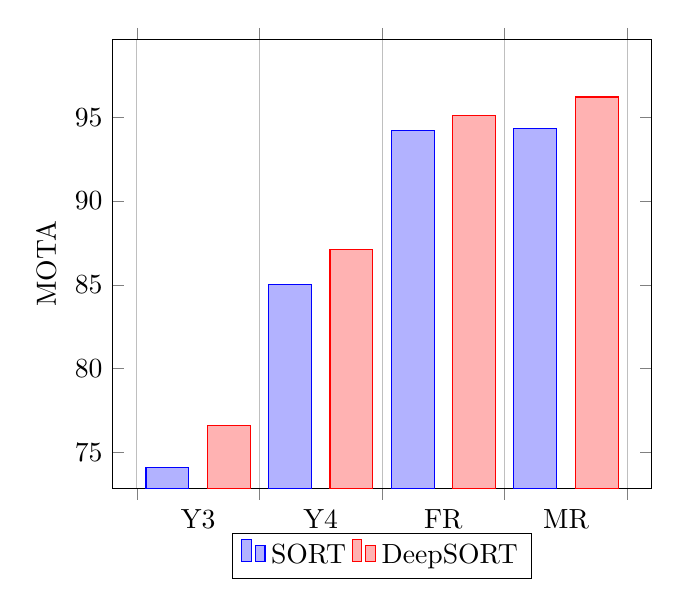
\begin{tikzpicture}
	\label{fig:pgf_mota}
	\begin{axis}[
		symbolic x coords={Y3,Y4,FR,MR,GT},
		x tick label style={
			/pgf/number format/1000 sep=},
		xlabel=Detection Algorithm,
		ylabel=MOTA,
		enlargelimits=0.05,
		legend style={at={(0.5,-0.1)},
			anchor=north,legend columns=-1},
		ybar interval=0.7,
		]
		\addplot 
		coordinates {(Y3,74.1) (Y4,85)
			(FR,94.2) (MR,94.3) (GT,97.5)};
		\addplot 
		coordinates {(Y3,76.6) (Y4,87.1)
			(FR,95.1) (MR,96.2) (GT,98.4)};
		\legend{SORT,DeepSORT}
	\end{axis}
\end{tikzpicture}
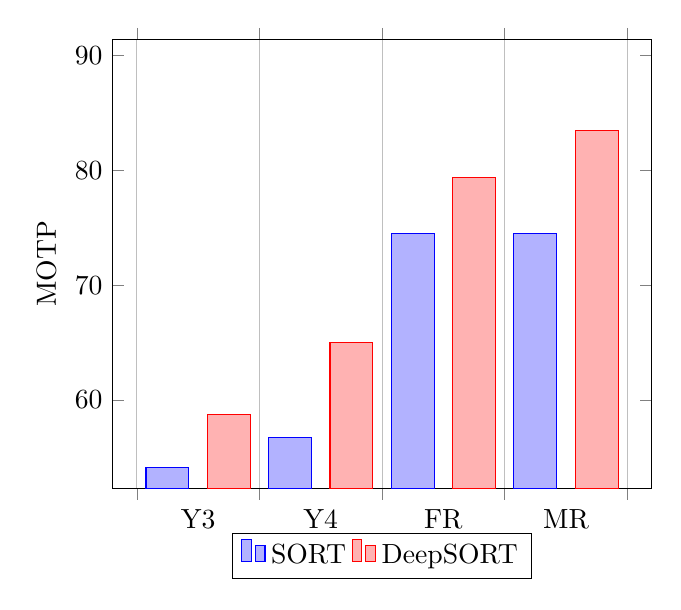
\begin{tikzpicture}
	\label{fig:pgf_motp}
	\begin{axis}[
		symbolic x coords={Y3,Y4,FR,MR,GT},
		x tick label style={
			/pgf/number format/1000 sep=},
		xlabel=Detection Algorithm,
		ylabel=MOTP,
		enlargelimits=0.05,
		legend style={at={(0.5,-0.1)},
			anchor=north,legend columns=-1},
		ybar interval=0.7,
		]
		\addplot 
		coordinates {(Y3,54.1) (Y4,56.7)
			(FR,74.5) (MR,74.5) (GT,89.1)};
		\addplot 
		coordinates {(Y3,58.7) (Y4,65)
			(FR,79.4) (MR,83.5) (GT,89.6)};
		\legend{SORT,DeepSORT}
	\end{axis}
\end{tikzpicture}
\caption{Overall MOTA and MOTP metric on Micand32E.}
\end{figure}
\subsection{Impact of detection method over tracking result}
In the sub-section \ref{subsec:det_res}, the accuracies of the Yolo family models and RCNN family models are reported and we insists that in term of precision, the MaskRCNN and FastRCNN completely outperforms the Yolos. The impact of choosing detection tactic on the tracking performance is also shown clearly in Figure 4 1 and Figure 4 2. On the same tracking method, SORT, MOTA results of Yolov3, Yolov4, FasterRCNN, MaskRCNN and detection groundtruth are respectively 74,1\%, 85\%, 94,2\%, 94,3\% and 97,5\%. Also it’s remarkable that the number of FN decreases, 3176 for Y3DS, 1581 for Y4DS, 282 for FDS, 184 for MDS and 82 for GDS. 
After researching theory and evaluating experiments, it’s quit intuitive but reasonable to conclude that the better detction method is, the higher tracking quality is.
\subsection{Complexsity of 4 types of patients's actions}
The diversity and comlexsity of 4 type of patient’s actions are analysed via metrics in Table \ref{tab:long_gds}, the highes results achived in this experiment. In term of MOTA metric, the GDS obtains best performance on the action type 6, with 2 sequences:  GH010373\_6\_3150\_4744 99,7\% and GH010358\_6\_10208\_11900 99\%. In the contrary, the MOTA for GH010358\_8\_8000\_5447 is 96,1\% with GDS.
On the other hand, the sequence’s volume also has impacts on the tracking qualities. All videos in Micand32S is short-term and the results of all the 11 aproaches is almost perfect on this datasets. But in Micand32E, the sequences is long and then many weaknesses of tracking algorithms appear, it’s visible via the metrics like IDP and IDR. However, on both datasets, almost aproaches can still track hands well, this is shown by metric GT and MT in Table \ref{tab:long_overall}.
\subsection{Challenging cases}
According to my personal coding experience through this thesis, multiple object tracking is quit difficult to debug errors. The evaluation process is not reversible, when the results are available, the mtrics can be calculated, but by just looking at metrics, it’s hard to known where the errors occur, we can only visualing the result through visible video to find the bug. In this way, I finds some challenging cases in some sequences that make almost of 11 approaches yeild tracking errors. Some typical cases are: (1) when the hands move quickly so that the cameras can’t catch, this make the frame motion blur; (2) when the shape of the hands changes heavily; (3) when hands occluded by other obstacles; (4) when the hands dissappear from the camera’s view and return after that.